\section{Tectonic model}
\label{sec:tectonicmodel}
We now introduce the detailed description of the tectonic model used to create the planet crust. We discuss differences and similarities with respect to the original article and adapt the mechanisms to our unit sphere representation. Parameters that drive the model are summarized at the end of the section in Table \ref{tab:model-parameters-summary}. It should be stated that all parameters will be optimized for the number of vertex samples $N$ equal to 500,000.

The simplest description of the algorithm is that it creates some random crust partitioning into plates. These plates have randomized drifting parameters for moving. Then a certain number of tectonic steps is performed with a time step length $\delta t$ of 2 My and the result is a basic crust of the simulated planet. Between automated tectonic steps, user can force a few specific interactions (plate rifting, terrain smoothing) and change various global parameters to influence the simulation. The planet radius is set to $6370\mbox{ km}=6.37\mbox{ u}$.
\subsection{Workflow}
Basic crust is generated from a Delaunay triangulation of a unit sphere. The fresh crust is just a set of triangulated vertices, while each vertex is assigned some default crust data $h$. Each tectonic step consists of several substeps in a sequence. This sequence is firmly set because of implementation context and is depicted in Figure \ref{fig:tectonic-step-structure}. Short descriptions for the substeps follow.
\begin{figure}[ht]
\centering
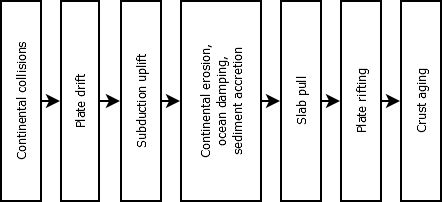
\includegraphics[width=12cm]{tectonic-step-structure.png}
\caption{Tectonic step structure}
\label{fig:tectonic-step-structure}
\end{figure}
\begin{itemize}[\label={}]
\item[\textbf{Continental collisions}] If the plate drift would result in an overlap of two different continental (above sea level) areas of crust belonging to different plates, a continental collision is triggered, resulting in a~massive uplift of the lighter plate. The two plates in question are then merged into one. This is different from the orignal algorithm, which only attaches connected continental areas, called \textit{terranes}.
\item[\textbf{Plate drift}] Rotation transform of each plate along the sphere surface is updated by its respective angular speed.
\item[\textbf{Subduction uplift}] Overlapping areas of different plates cause uplift in the lighter plates. This process is known as \textit{subduction}. Note that overlapping continental areas have already been dealt with so this case should never occur during this step.
\item[\textbf{Continental erosion, ocean damping, sediment accretion}] This step updates elevation values to simulate erosion of crust above sea level, lowering of the ocean bottom for underwater crust and sediment accretion for the ocean crust below average ocean depth. This is questionable, as the original algorithm probably detects trench area for sediment filling.
\item[\textbf{Slab pull}] Subducting parts of plates tend to pull the plate towards them, altering the surface rotation. All vertices in subduction zones contribute to the rotation vectors of their plates.
\item[\textbf{Plate rifting}] Every tectonic step the largest plate has a chance to rift apart. Along some random linear border within the plate the vertices are assigned to two new plates with diverging velocities.
\item[\textbf{Crust aging}] Age of every crust vertex is updated by the length of the tectonic step.
\end{itemize}
\subsection{Crust \& plates}
The crust is defined as a set of surface vertices $U$, obtained by Fibonacci sampling. Its size is the number of samples $N$. Each vertex $\mathbf{u}_i\in U$ is assigned crust point data $h_i$. The tectonic plate system is an~equivalence system $\mathcal{P}$ of $U$ (so that every crust point belongs exactly to one plate). These equivalence classes should be connected through the mesh, but it is not a strict requirement (although it subtracts from the realism). Plates are the individual equivalence classes $\mathcal{P}_i\in\mathcal{P}$. If all vertices of a~mesh triangle belong to a~plate $\mathcal{P}_i$, the triangle is also said to belong to $\mathcal{P}_i$. A triangle only has three neighbours, each sharing one edge. If a triangle belonging to $\mathcal{P}_i$ has a neighbouring triangle which does not, it is called a \textit{border triangle}.

Each plate is also assigned: a centroid $\mathbf{c}_i$, rotation axis $\mathbf{w}_i$, plate angular speed $\omega_i$ and a transform $q_i$. The centroid is a vector calculated as the normalized sum of all vector representations of vertices belonging to the plate. If it cannot be normalized, a random vector is assigned. The rotation axis is a unit vector along the axis around which the plate drifts. The plate angular speed is self-explanatory. The transform is a quaternion representation of the relative rotation of the plate with respect to the original position. This is because the simulation does not actually move the plate vertices, only adjusts the plate transform to correctly calculate interactions. Moving the vertices would introduce serious problems with rendering.
\subsection{Crust data}
Crust data values included so far are: elevation, crust thickness, orogeny type and crust age. All crust points are strictly represented by unit vectors. The elevation values are information stored separately. Ocean crust are all crust points with negative elevation, continental crust points have a non-negative elevation. Crust thickness is a placeholder information for potential future updates. Orogeny type is represented by three categories: \textit{None}, \textit{Andean} and \textit{Himalayan}. The Andean type is a crust point elevated above the ocean level by subduction, the Himalayan type is a crust point that was influenced by continental collision. The None type is reserved for crust points not yet elevated by continental collision nor elevated above the ocean level by subduction. It does not exist in the original article, as the orogeny type is reserved for continental crust. The crust age is simple the time passed from the creation of the crust point. The original model also uses fold direction, which is not yet implemented, as I do not properly understand its purpose and mechanics.

The default crust point data for new points depends on whether the new point is continental or not. The only new continental points are created during the first partitioning (see Subsection \ref{subsec:plate-initialization}). Initial elevation is $z_{0t}=-0.004 \mbox{ u}$ for ocean crust and $z_{0c}=0.001 \mbox{ u}$ for continental crust. Crust thickness is always calculated from a~basic crust thickness value $e_0=0.01\mbox{ u}$ as $e=e_0+z$, where $z$ is the crust elevation. The initial orogeny type is None for all new ocean crust points and Andean for the initial continental crust. Initial crust age is universally equal to 0.
\subsection{Plate initialization}
\label{subsec:plate-initialization}
Partitioning of the crust into the initial set of plates  is governed by two parameters: the number of initial plates $N_\mathcal{P}$ and the probability of an initial plate being continental $p_C$. The initial number of plates is 40 and the probability of an initial plate to be continental is 0 for testing purposes. Before partitioning, vector noise is assigned to each triangle on the mesh with a noise averaging iterations parameter $n_{\mbox{sm}}$ of 4.

At first, $N_\mathcal{P}$ number of random points $\mathbf{c}$ (future \textit{centroids} of the plates) is distributed on the surface. Then all initial crust vertices are assigned to these points by their shortest distance on a unit sphere:
$$d(\mathbf{x},\mathbf{c})=\arccos(\mathbf{x}\cdot\mathbf{c})$$
All points that have the shortest distance to a certain centroid point belong to a single plate. This plate inherints the points and the centroid. When all points are distributed to their plates, each plate is then assigned a random rotation axis $\mathbf{w}$ and random non-negative angular speed $\omega$. The maximum plate angular speed is $v_0=0.0157\mbox{ My}^{-1}$. The symbol is unchanged to correspond with the original quantity. Finally, each plate is assigned a quaternion identity transform $q$. All crust points are assigned default data according to their plate. The probability of continental crust is evaluated on the plate level, so the initial plates all have the same elevation.

This kind of initialization basically creates a Voronoi diagram with perfectly straight lines (up to the triangle resolution). To simulate more realistic plate boundaries, vector noise is used. First we look for the triangles which have vertices from exactly two different plates. For each of these triangles we try to roll for probability equal to its noise vector magnitude. If the probability succeeds, we compute three dot products between the noise vector and each vector from the triangle barycenter to the vertex. The vertex with the maximum dot product is assigned to the plate of the vertex with the minimum dot product. This shifts the borders of the plates and is repeated $n_{\mbox{vb}}=4$ times. This parameter is the number of Voronoi border shift iterations. An example of the resulting partitioning can be seen in Figure \ref{fig:initial-plates}.
\begin{figure}[ht]
\centering
\begin{subfigure}{7cm}
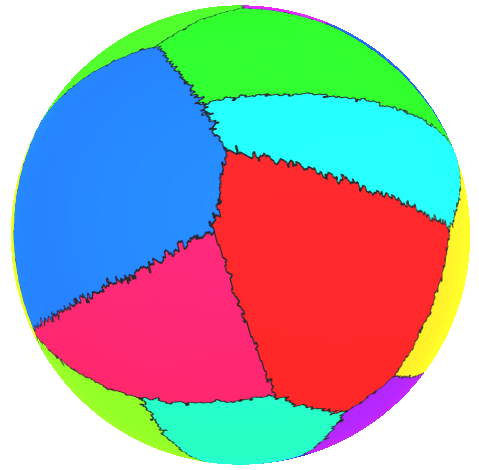
\includegraphics[height=7cm]{plate-initialization.png}
\caption{initial plates}
\label{fig:initial-plates}
\end{subfigure}
\hspace*{1cm}
\begin{subfigure}{7cm}
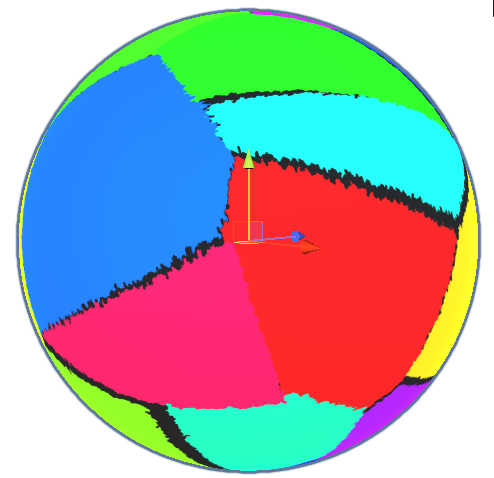
\includegraphics[height=7cm]{plate-drift.png}
\caption{plates drifting}
\label{fig:plates-drifting}
\end{subfigure}
\caption{Crust partitioning}
\label{fig:crust-partitioning}
\end{figure}
\subsection{Plate overlaps}
Tectonic interactions require the concept of plate density. For example, denser ocean plates are subducted under continental plates. Because our model does not have a clear designation of a plate as ocean or continental (any plate can have ocean or continental crust), we evaluate plates by a weighted sum of their vertices. Each plate is assigned a score equal to:
$$\mbox{score}=100\times\mbox{number of continental crust points}-\mbox{number of ocean crust points}$$
The plates are then ranked by the highest score. The rank decides which plate 'goes under' when two plates overlap (the one with a lower score). This actually creates an irreflexive, antisymmetric and transitive relation on the set of plates.

This ranking system is a gross simplification. As many simplifications, though, it makes certain decisions and calculations much easier. The plate ranks have to be recalculated every time an interaction requires them, as the scores change both with crust elevation and changes in crust point assignments to plates. An example might be when we need to know which of the overlapping plates defines a crust point elevation on the surface.
\subsection{Plate drift}
The main reason for tectonic interactions is the tectonic drift. Plates move constantly, causing collisions, subduction etc. To model the drift of a plate, during every tectonic step the plate transform is adjusted
by multiplication of the transform by a quaternion representing a rotation around the axis $\mathbf{w}$ by the angle of $\Delta\phi=\omega\delta t$. This keeps the information about current crust points locations. The result of a one step drift from the initial position can be seen in Figure \ref{fig:plates-drifting}. We can see here that the plates move as individual rigid bodies.
\subsection{Ocean crust generation \& crust resampling}
Moving rigid plates necessarily create gaps on the surface. In reality, this 'empty' space is filled with new crust drifting from ocean ridges between the plates (see Figure \ref{fig:resample-mesh}). We use the original model, only slightly simplified. We can interpolate crust data at any point on the surface which is not in any triangle belonging to a plate. We compute two distances to two nearest plates (nearest vertices belonging to two different plates) $d_1$ and $d_2$ (1 being the absolute shortest) and assume that the point is approximately on the direct line between the nearest points. We also assume that the ridge is directly in the middle of the line. This is not true in reality, but makes it simple to use the original algorithm easily. We compute the ridge and plate elevation contributions and combine them as per Cortial et al.
\begin{figure}[ht]
\centering
\begin{subfigure}{7cm}
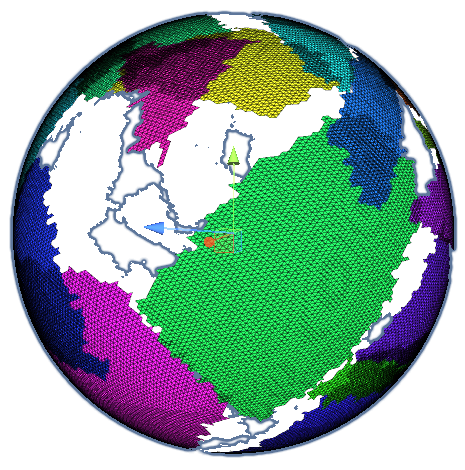
\includegraphics[height=7cm]{resample-drift.png}
\caption{diverging plates}
\label{fig:resample-drift}
\end{subfigure}
\hspace*{1cm}
\begin{subfigure}{7cm}
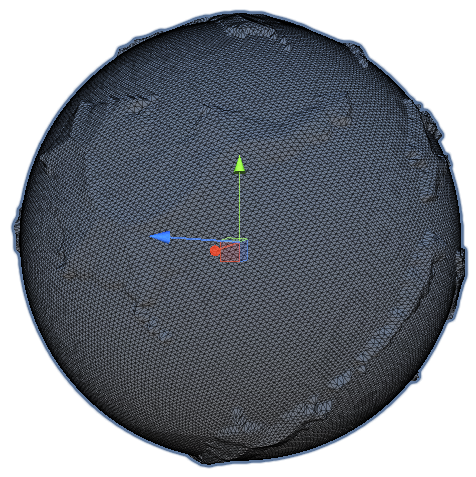
\includegraphics[height=7cm]{resample-ridges.png}
\caption{generated ridges}
\label{fig:resample-ridges}
\end{subfigure}
\caption{Ocean crust generation}
\label{fig:resample-mesh}
\end{figure}

The ridge function profile uses three parameters: the highest ocean ridge elevation $z_r$, the abyssal plains elevation $z_a$ and the ocean ridge elevation falloff $\sigma_r$. The values of these parameters are:
$$z_r=-1\mbox{ km}=-0.001\mbox{ u}$$
$$z_a=-6\mbox{ km}=-0.006\mbox{ u}$$
$$\sigma_r=0.05\mbox{ u}$$
The ridge function profile is a function of a variable $d_\Gamma$ which is the distance to the ocean ridge. The function profile is chosen as:
$$z_\Gamma=(z_r-z_a)2^{\frac{d_\Gamma}{\sigma_r}}+z_a$$
The original function profile is not specifically described and may be more complex.
Because of our assumptions we can calculate the ridge function profile variable that is the distance to the ridge as:
$$d_\Gamma=\frac{d_2-d_1}{2}$$
The orogeny type is universally filled as None for points in the surface voids. The crust age is computed as the scaling parameter $\alpha=\frac{d_\Gamma}{d_\Gamma+d_1}$ multiplied by the total time for which the plates have been diverging (since last they were in close contact). This makes the new ocean crust gradually older the further it is from the ridge. Finally, any new ocean crust point is assigned to the nearest plate.

For simulation running for many steps it is vital that we periodically resample the surface to fill the gaps made by diverging plates and to resolve overlapping plates. As per Cortial et al., it is recommended to resample the surface every 10th-60th step. Our model forces resampling on several occasions, namely continental collision. The resampling simply means to interpolate surface data onto the original mesh from the current surface data defined on a mesh broken by drifting plates and interactions. For each initial mesh vertex, we test if it is found on a plate with the highest rank possible. If so, we perform barycentric interpolation from a triangle within which the vertex currently resides. If no plate is found, we create a new ocean crust point.
\begin{table}[h]
\centering
\begin{tabular}{cccc}
\textbf{Symbol}&\textbf{Description}&\textbf{Original value}&\textbf{Model value}\\
\hline
$N$&Number of mesh vertices&-&500,000\\
$\delta t$&Tectonic time step&2 My&2 My\\
$R$&Planet radius&6,378 km&6.37 u\\
$z_{0t}$&Initial ocean elevation&-&-0.004 u\\
$z_{0c}$&Initial continental elevation&-&0.001 u\\
$e_0$&Basic crust thickness&-&0.01 u\\
$N_\mathcal{P}$&Initial number of plates&-&40\\
$p_C$&Initial continental plate probability&0.3&0\\
$v_0$&Maximum plate speed&100 mm$\cdot$y$^{-1}$&$0.0157\mbox{ My}^{-1}$\\
$n_{\mbox{sm}}$&noise averaging iterations&-&4\\
$n_{\mbox{vb}}$&Voronoi border shift iterations&-&4\\
$z_r$&Highest ocean ridge elevation&$-1\mbox{ km}$&$-0.001\mbox{ u}$\\
$z_a$&Abyssal plains elevation&-6\mbox{ km}&$-0.006\mbox{ u}$\\
$\sigma_r$&Ocean ridge elevation falloff&-&0.05\mbox{ u}\\
\end{tabular}
\caption{Model parameters summary}
\label{tab:model-parameters-summary}
\end{table}